\chapter{Prototypische Implementierung}
\label{chap:impl}
Dieses Kapitel widmet sich der prototypischen Implementierung der im vorigen Kapitel vorgestellten Konzeption des Frameworks. Als Vorgabe wird diese in  C++ entwickelt. Das UML-Klassendiagrammes in \Fref[plain]{fig:uml} spiegelt den groben Aufbau wieder und zeigt die wichtigsten Klassen. Auf die Darstellung von Hilfskonstrukten wird der Übersichtlichkeit verzichtet. Als erster Schritt wird die Anbindung an die Netzwerke erklärt. Danach wird -- ausgehend von der Applikation -- die Implementierung des Publish/Subscribe-Systems erläutert. Angewandte Techniken wie \ac{tmp} oder \emph{policy based}-Design werden im Anhang dieser Arbeit beschrieben. Sie werden benötigt um den zusätzlichen Verwaltungsaufwand zur Laufzeit durch geschickte Anwendung des zur Übersetzungszeit vorhandenen Wissens zu minimieren. Das nutzbare Wissen umfasst beispielsweise die Typen der Events oder die zur Optimierung ausgewählten Strategien und deren Besonderheiten.

\texttt{P2PInterface} ist eine abstrakte Basisklasse und repräsentiert die in \cite{Dabek2003Towards} beschrieben KBR-API. Aktuell wird diese durch die Klasse \texttt{ChimeraWrapper} implementiert, welche über die Klasse \texttt{ChimeraWrapperImpl} Zugriff auf das Netzwerk Chimera bietet. Hier wurde das ``PIMPL''-Pattern angewandt, mit dem die eigentliche Implementierung versteckt werden kann \cite{Alexandrescu2001Modern}. Zur Vereinfachung werden sämtliche Identifikationsdaten, zum Beispiel die Adresse eines Knotens, des Netzwerkes als \texttt{std::string} repräsentiert. Dies entbindet den Entwickler der Implementierung weiterer Wrapperklassen von komplexen Hilfskonstrukten. Zur eigentlichen Nachrichtenübertragung wird der Datentyp \texttt{std::vector$<$char$>$}, die objektorientierte Version eines \texttt{char*}, bereitgestellt. Neben der einfacheren Zugriffsweise, bietet dies zusätzlichen Schutz gegen einen Bufferüberlauf und ähnliche Probleme.\\
Weitere Netzwerke können auf einfache Art und Weise durch entsprechende Wrapperklassen eingebunden werden.

\begin{figure}[htbp]
\centering
\resizebox{\textwidth}{!}{%
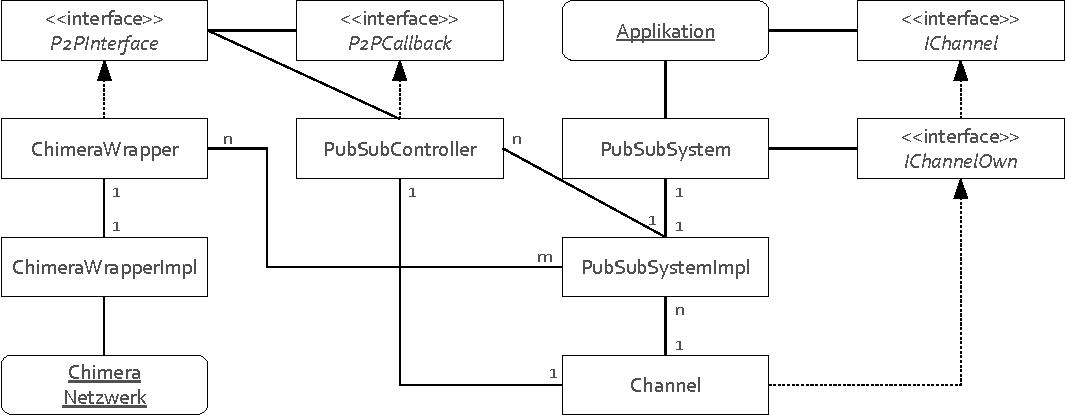
\includegraphics{grafics/uml.pdf}}
\caption{vereinfachtes Klassendiagramm des Frameworks}
\label{fig:uml}
\end{figure}

Die \texttt{Applikation} greift auf das Publish/Subscribe-System über den Singleton \texttt{PubSub\-Sytem} zu. Beiden ist der optimierte \texttt{Channel} nur über die abstrakten Basisklassen \texttt{IChannel} beziehungsweise \texttt{IChannelOwn} zugänglich. Diese bieten lediglich die drei üblichen Methoden\footnote{subscribe, unsubscribe und publish} für Publish/Subscribe-Systeme an und verdecken dadurch die Komplexität der Klasse Channel vor dem Benutzer. Channel selbst ist eine mit policy-based Design erstellte Templateklasse\footnote{siehe \Fref{chap:impl_tmp} im Anhang zur Erklärung} und bekommt die verschiedenen Strategien -- in \Fref{fig:uml} ebenfalls nicht dargestellt -- als Policies übergeben. \ac{tmp} ermöglicht es zudem jeden Channel auf die gewählten Policies abzustimmen. Weiterhin wird für jeden Channel ein optimierten Header erzeugt, dessen Größe an Nutzlast für Verwaltungsdaten von den gewählten Policies abhängig ist. Durch diese Maßnahmen wird der Overhead zur Laufzeit stark reduziert. 

Die Klasse \texttt{PubSubController} implementiert das Interface \texttt{P2PCallback} und kann sich somit für die Callbacks des Netzwerkes registrieren. Der PubSubController ist die Schnittstelle des Publish/Subscribe-Systems mit dem \ac{p2p}-Netzwerk und bietet die benötigte Funktionalität für die Klasse Channel. Zudem werden die ankommenden Nachrichten in deliver über eine Queue und einen Dispatch-Thread an die einzelnen Kanäle verteilt. 

\texttt{PubSubSystemImpl} kennt die verschiedenen Netzwerkwrapper (in \Fref{fig:uml} ist dies ChimeraWrapper) und besitzt für jeden optimierten Channel eine Klassenvariable als IChannelOwn*. Auf diese hat die Klasse PubSubSystem als \texttt{friend class}\footnote{``friend'' ist eine besondere Beziehung zwischen zwei Klassen} freien Zugriff und kann die Methodenaufrufe an der Publish/Subscribe-API an die Kanäle weiterleiten. Für jedes genutztes Netzwerk instantiiert PubSubSystemImpl einen PubSubController und übergibt diesen an die entsprechenden Channel. Mit verschiedenen Instanzen der Klasse PubSubController können somit auch verschiedene Netzwerke angesprochen werden und entsprechend der Optimierungsmetriken für verschiedene Kanäle genutzt werden.\\

Im Optimierungsschritt müssen folgende Klassen generiert oder teilweise angepasst werden:
\begin{description}
\item[ChannelList.h] In dieser Datei ist eine Liste der vorhandenen Kanäle in einem \texttt{enum} abgelegt. Die Einträge dienen der Auswahl des Kanals bei der Kommunikation mit dem PubSubSytem. Durch das enum wird ein einfach zu überprüfendes Mapping auf den eigentlichen Kanal ermöglicht.
\item[PubSubSystemImpl.h] Diese Klasse muss komplett generiert werden. Sie hat Zugriff auf alle zur Optimierung genutzten Strategien und den daraus erzeugten Instanzen der Templateklasse Channel. Zudem können hier die verschiedenen Netzwerke mit den verschiedenen Kanälen über Instanzen der Klasse PubSubController verbunden werden.
\item[PubSubSytem.cpp] Die Klasse PubSubSystemImpl und damit auch die optimierten Kanäle werden erst im Optimierungsschritt erzeugt. Daher müssen die Zugriffsmethoden auf die im PubSubSystemImpl enthaltenen Kanäle ebenfalls im Optimerungsschritt generiert werden.
\end{description}

Dank der strikten Aufteilung der Klassen beim Netzwerk und dem Publish/Subscribe-System wird die Nutzerfreundlichkeit des Frameworks aus Entwicklersicht ermöglicht, wie es das Codebeispiel im nächsten Abschnitt darlegt. Hier ist deutlich zu sehen, dass der Nutzer keinerlei Wissen über das genutzte Netzwerk, noch über die zur Optimierung herangezogenen Strategien haben muss um das System benutzen zu können.

\section*{Zugriff auf M$^2$etis aus Benutzersicht}
Das \Fref{lst:pubsub_usage} zeigt den Zugriff der Applikation auf das Publish/Subscribe-System. Der Code erzeugt drei Knoten, die mit dem System arbeiten. Der erste Knoten sendet Nachrichten auf dem Kanal \texttt{BROADCAST}, für den sich die beiden anderen Knoten anmelden. In den Zeilen 10 bis 12 ist die Empfangsfunktion definiert, welche dem System bei Anmeldungen übergeben werden muss. Diese Funktion wird in den Zeilen 18 und 21 mittels \texttt{boost::bind} an die benötigte Signatur angepasst und mit Metadaten (hier der Knotenname) angereichert. In den Zeilen 15 und 16 wird das System initialisiert und ein Handle auf den Kanal \texttt{BROADCAST} erlangt. Die Anmeldung der Knoten erfolgt in den Zeilen 19 und 22, mit Angabe des eines im Netzwerk bekannten Knoten zum Einstieg in das Netzwerk und der Empfangsfunktion. In den Zeilen 24-27 wird in einer Endlosschleife eine Nachricht über das Handle in das System gebracht und fünf Sekunden geschlafen.

Dieses Codebeispiel zeigt deutlich die Kapselung des komplexen optimierten Publish/\-Subscribe-Systems und dessen einfache und unkomplizierte Handhabbarkeit. Über \texttt{boost::bind} können beliebige Methoden an die Signatur der Empfangsfunktion angepasst werden. Daher muss die Applikation einerseits nicht von einer abstrakten Basisklasse abgeleitet sein und andererseits bleibt die eigentlich Empfangsfunktion anpassbar wie es im Codebeispiel dargestellt ist.

\lstinputlisting[caption={Zugriff auf M$^2$etis aus Benutzersicht}, label=lst:pubsub_usage]{listings/pubsub_usage.cpp}


